\chapter{REDES NEURAIS ARTIFICIAIS}
\label{chap:ann}
%quad = paragrafo \\ pula linha
\quad Redes neurais artificiais são estruturas matemáticas capazes de aprender, memorizar e generalizar determinadas situações e problemas a ela apresentado. Rede neural é inspirada no cérebro e é formada por neurônios que se ligam entre si e de acordo com uma determinada função, realizam sinapses entre si \cite{hay}.\\

Em 1943 o psiquiatra e neuroanatomista Warren McCulloch e o matemático Walter Pitts propuseram um modelo matemático de um neurônio artificial. O modelo era uma simplificação do neurônio biológico representado na Figura \ref{fig:neur}. 

\begin{figure}[H]
\centering % para centralizarmos a figura
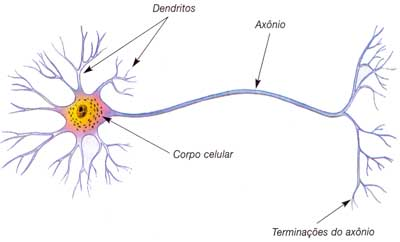
\includegraphics[width=10cm]{img/neuronio.jpg} % leia abaixo
\caption{Estrutura básica de um neurônio biológico. \textit{fonte:\cite{barroso}}}
\label{fig:neur}
\end{figure}

Para representar os dendritos, o modelo usou $n$ terminais de entrada de informações $x_1, x_2, x_3, \dots, x_{n-1}, x_n$ e um terminal de saída $y$ representando o axônio. As sinapses são  simuladas de acordo com um coeficiente ponderador, a sinapse só ocorre quando a soma ponderada dos sinais de entrada ultrapassa um limiar pré-definido. Este limiar é chamado de função de ativação e foi definido de forma Booleana. A Figura \ref{fig:ann} mostra o neurônio artificial.

\begin{figure}[H]
\centering % para centralizarmos a figura
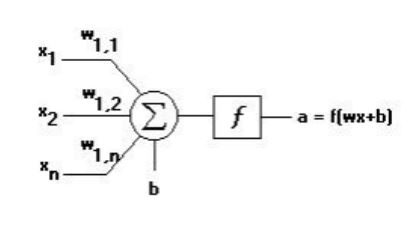
\includegraphics[width=10cm]{img/neura.jpg} % leia abaixo
\caption{Neurônio artificial proposto por McCulloch e Pitts. \textit{\cite{fia}} }
\label{fig:ann}
\end{figure}

A equação \ref{eq:neu} é a equação da saída $y$ do neurônio.
\begin{equation}\label{eq:neu}
y = f \Big(\sum_{i=1}^{n}x_iw_i +b\Big)
\end{equation}
Onde $n$ é o número de entradas do neurônio, $w_i$
 é o peso associado à entrada $x_i$ e $f$ é a função de ativação utilizada. 


\section{Classificação de Redes Neurais Artificiais}
\label{sec:class}
\quad Redes neurais podem ser classificadas de acordo com a topologia ou a forma de aprendizagem. Estas classificações são explicadas nas seções \ref{sec:top} e \ref{sec:lear} respectivamente.

\subsection{Topologia}
\label{sec:top}
As RNAs podem ser classificadas de acordo com sua topologia em:
\begin {enumerate}
\item Perceptron de Camada Única: É utilizado para classificação linear, ou seja, utilizada em problemas que sejam linearmente separáveis. A Figura \ref{fig:ann1} mostra um exemplo de perceptron de camada única;
\begin{figure}[H]
\centering % para centralizarmos a figura
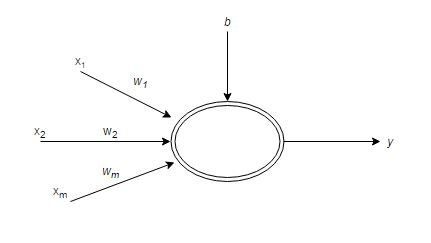
\includegraphics[width=10cm]{img/rna1.jpg} % leia abaixo
\caption{Perceptron de camada única.}
\label{fig:ann1}
\end{figure}
\item Perceptron de Múltiplas Camadas: Possui várias camadas, e possuem, camadas ocultas, onde dentro delas, esta inserindo neurônios ocultos, ou seja recursos computacionais.  A Figura \ref{fig:annm} mostra um exemplo de perceptron de várias camadas;

\begin{figure}[H]
\centering % para centralizarmos a figura
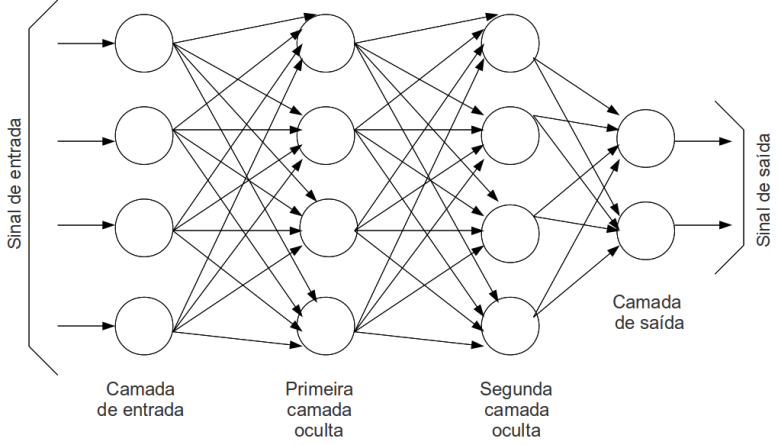
\includegraphics[width=10cm]{img/annm.png} % leia abaixo
\caption{Perceptron de múltiplas camadas.}
\label{fig:annm}
\end{figure}

\item Redes Recorrentes: Possui pelo menos um laço de realimentação, pode ser implementada tanto no perceptron de camada única,  como, no perceptron de multicamadas.  A Figura \ref{fig:annrec} mostra um exemplo de perceptron recorrente;

\begin{figure}[H]
\centering % para centralizarmos a figura
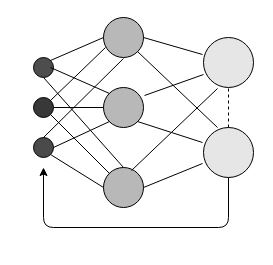
\includegraphics[width=10cm]{img/rnarea.jpg} % leia abaixo
\caption{Perceptron recorrente.}
\label{fig:annrec}
\end{figure}


\end{enumerate}

\subsection{Tipos de Aprendizagem}
\label{sec:lear}
Outra maneira de classificar redes neurais é de acordo com o tipo de aprendizagem. Esta pode ser:
\begin {enumerate}
\item Aprendizagem Supervisionada: Há uma amostra  que será comparada ao ambiente.
\item Aprendizagem Não Supervisionada: Procura-se um padrão, sem a ajuda de uma amostra de comparação. Essas redes são chamadas de mapas auto-organizáveis, estes são explicados na seção \ref{sec:som}.
\end {enumerate}


\section {SOM - Self Organizing Maps}
\label{sec:som}
\quad  De acordo com \cite{ia}  um mapa auto-orgánizavel é estruturado pelo neurônio vencedor de uma competição, ditada por uma função discriminante de cada iteração, também chamada de época. Essa competição pode ser em neurônio contra todos os neurônios da rede, ou, neurônio contra um grupo de neurônios da rede. Um das metas de um mapa auto-organizável é classificar os dados de entrada competindo entre si. O algoritmo possui um conjunto de regras de natureza local. O termo local significa que a modificação aplicada ao peso sináptico de um neurônio é confinada à vizinhança imediata daquele neurônio.

\section { Alguns principios intuitivos de auto-organização}
\quad A organização da rede acontece em dois níveis diferentes, que interagem entre si na forma de um laço de realimentação.  De acordo com \cite{hay} os dois niveis são:
\begin{itemize}
\item  Atividade: Certos padrões de atividade são produzidos por uma determinada rede em resposta a sinais de entrada.
\item Conectividade: Forças de conexão dos pesos sinápticos da rede  são modificadas em resposta a sinais neurais dos padrões de atividade. 
\end{itemize}

Pode-se citar, ainda de acordo com \cite{hay}, que mapas auto-organizáveis possuem os seguintes princípios:
\begin{itemize}
\item  Modificações dos pesos  sinápticos tendem a se auto-amplificar. Para estabilizar o sistema, deve haver alguma forma de competição por recursos limitados. Especificamente, um aumento na força de algumas sinapses da rede deve ser compensados por uma redução em outras sinapses.
\item  A limitação de recursos leva à competição entre sinapses e com isso à seleção das sinapses  que crescem mais vigorosamente  às custas das outras sinapses.
\item As modificações em pesos sinápticos tendem a cooperar.
\item Ordem e estrutura nos padrões de informação representam informação redundante que é adquirida pela rede neural na forma de conhecimento, que é um pré-requisito necessário para a aprendizagem.
\end{itemize}

\section{Mapa Auto-Organizável de Kohonen}
\label{sec:kohonen}
Os mapas auto-organizáveis foram desenvolvidos por Teuvo Kohonen em 1981 e fazem parte de um grupo de redes neurais baseadas em modelos de competição \cite{fia}. Uma característica importante destes mapas é que eles utilizam treinamento não supervisionado, os neurônios competem entre si e ajustam  seus pesos com base nesta competição. O principal objetivo dos mapas auto-organizáveis de Kohonen é agrupar os dados de entrada que são semelhantes entre si formando classes ou agrupamentos denominados \textit{clusters}. Segundo \cite{agua} os mapas de Kohonen podem ser aplicados para problemas não lineares de alta dimensionalidade, como por exemplo: processamento de sinais, demodulação e transmissão de sinais, extração de características e classificação de imagens e padrões acústicos, química e medicina. \\
Baseado no aprendizado competitivo, os mapas de Kohonen são do tipo \textit{winner-takes-all}, ou seja, \textit{o vencedor leva tudo}. Os neurônios de saída competem para serem ativados e a cada iteração apenas um neurônio é ativado. O funcionamento do SOM pode ser compreendido em diferentes etapas. A etapa competitiva na qual se define o neurônio mais adequado, chamado de \textbf{BMU} (\textit{do inglês Best Matching Unit}). A escolha da melhor correspondência entre o vetor de entrada e o vetor peso é feita por critério da menor distância euclidiana entre o vetor de pesos por ela armazenado e o vetor de entrada de acordo com a equação \ref{eq:euc} 
\begin{equation}
\label{eq:euc}
i(x)= argmin \big|x - w_j \big| \quad j = 1,2, \ldots n
\end{equation}
Onde $i(x)$ é a representação do neurônio da entrada $x$, e $w_j$ é o vetor peso. A função da  distância Euclidiana usada para 
quantificar a semelhança entre os vetores da rede é definida pela equação \ref{eq:euc2}.
\begin{equation}
\label{eq:euc2}
D_E = \sqrt{(x_1 - y_1)^2 + (x_2 - y_2)^2 + \ldots + (x_n - y_n)^2}
\end{equation}
Onde $x_n$ são as coordenadas dos vetores de entrada e $y_n$ são as coordenadas dos vetores  pesos  das redes auto-organozáveis.\\
Na etapa cooperativa os vizinhos são definidos dentro de uma distância obtida a partir da BMU. O processo de treinamento consiste na otimização da distância entre os neurônios. A vizinhança topológica é definida por meio da interatividade entre os neurônios. Um neurônio ativado tende a excitar os neurônios em sua vizinhança imediata. Cada iteração de atualização dos valores e distâncias da rede é chamada de época. As épocas constituem a  etapa adaptativa.


